\documentclass[a4paper,11pt]{article}

/stock/16_git_repo/library/library.tex
../../../../00_resources/page_garde.tex

\usepackage{fullpage}

\author{}
\title{}
\location{Montpellier}\blurb{}
\makeatother
\title{Devoir à rendre}
\author{Guillerme DUVILLIE}
\location{Montpellier}
\blurb{
    Université Montpellier II\\
    Master Informatique Modélisation, Optimisation Combinatoire et Algorithmique \\[1em]
    Matière : Cryptologie\\
    Encadrant : Christophe NEGRE
}

\begin{document}

\maketitle

\section*{Cryptanalyse différentielle}

Soit le $SPN$ à quatre rondes de la figure \ref{spn}, soit la boîte $S$ de substitution définie par
:
\begin{displaymath}
    \begin{array}{|c|cccccccc|} \hline
        X & [0,0,0,0] & [0,0,0,1] & [0,0,1,0] & [0,0,1,1] & [0,1,0,0] & [0,1,0,1] & [0,1,1,0] &
        [0,1,1,1] \\ \hline
        S(X) & [1,1,1,0] & [0,0,1,0] & [0,0,0,1] & [0,0,1,1] & [1,1,0,1] & [1,0,0,1] & [0,0,0,0] &
        [0,1,1,0] \\ \hline \hline
        X & [1,0,0,0] & [1,0,0,1] & [1,0,1,0] & [1,0,1,1] & [1,1,0,0] & [1,1,0,1] & [1,1,1,0] &
        [1,1,1,1] \\ \hline
        S(X) & [1,1,1,1] & [0,1,0,0] & [0,1,0,1] & [1,0,1,0] & [1,0,0,0] & [1,1,0,0] & [0,1,1,1] &
        [1,0,1,1] \\ \hline
    \end{array}
\end{displaymath}

et soit la permutation $P$ définie par : 
\begin{displaymath}
    P([u_1,\dots,u_{12}]) = [u_5, u_9, u_2, u_7, u_{10}, u_1, u_4, u_{11}, u_6, u_3, u_{12}, u_8]
\end{displaymath}

On cherche à réaliser une cryptanalyse différentielle sur le SPN décrit précédemment. Pour ce faire
il nous faut trouver une différence en entrée dont la probabilité de propagation soit maximale.
Intuitivement, on s'intéresse d'abord aux différences $\Delta$ en entrée et $\Delta^*$ de la boîte
$S$ dont la probabilité de propagation est maximale. Les valeurs de $N_{\Delta \rightarrow
\Delta^*}$ sont présentées dans le tableau~\ref{tabN}\footnote{Les résultats sont ceux trouvés par
le programme.}

\begin{figure}
    \begin{center}
        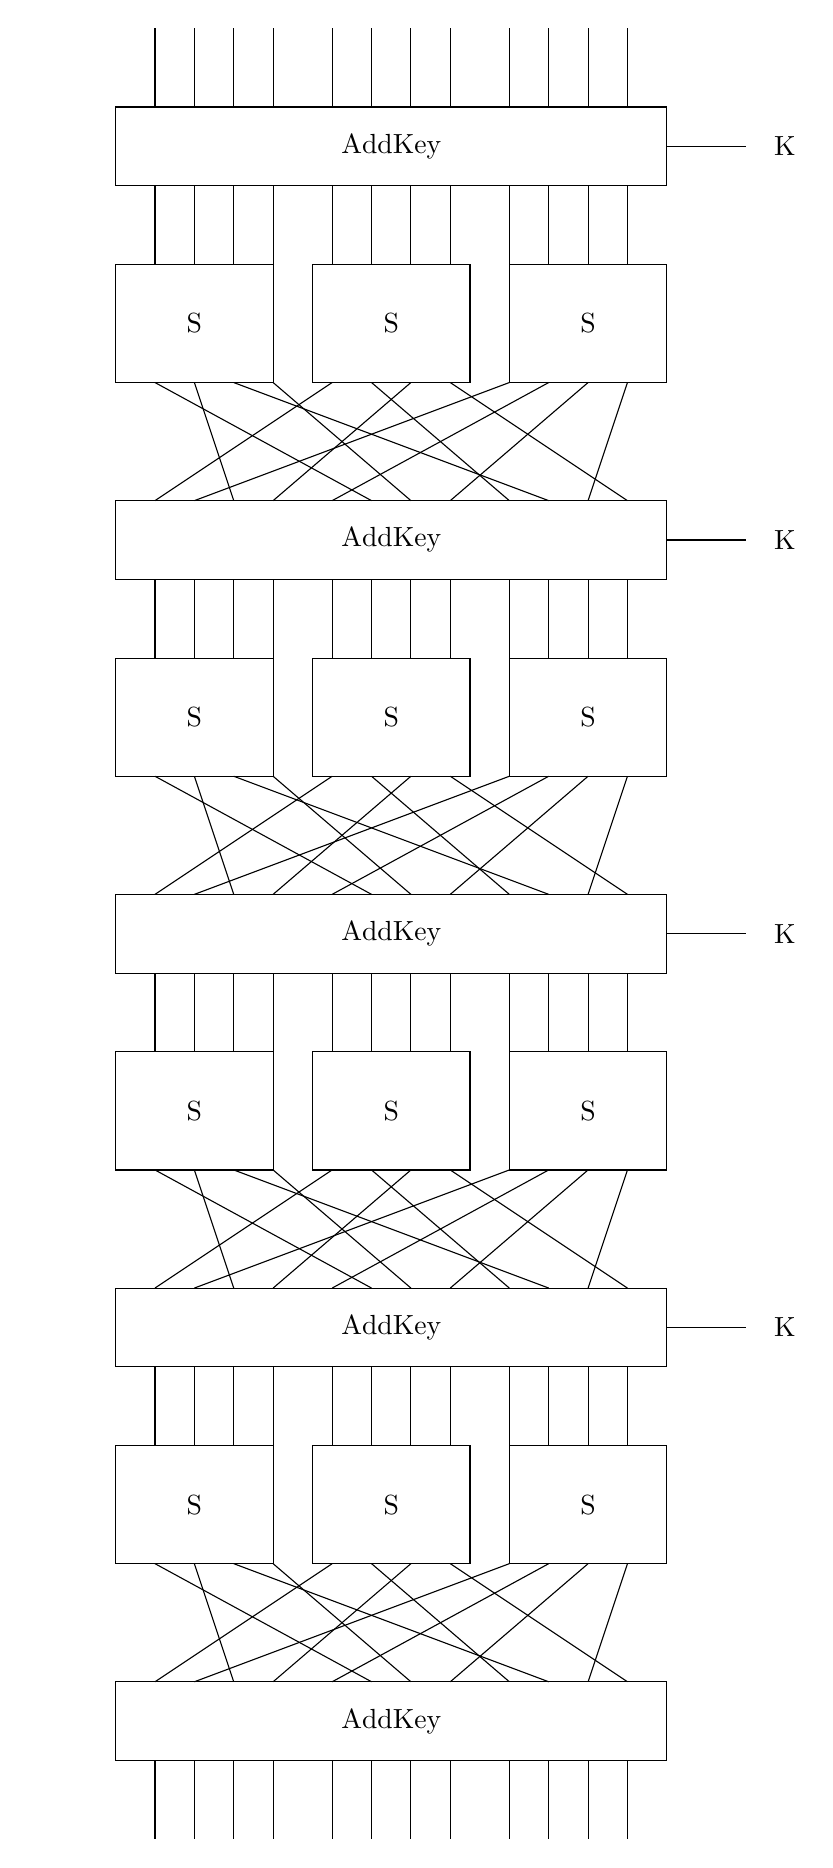
\begin{tikzpicture}[scale=0.50]
            \foreach \x in {1, 2, 3, 4, 5.5, 6.5, 7.5, 8.5, 10, 11, 12, 13}
                \draw[-] (\x, 33) -- (\x, 31);
            \foreach \y in {31, 21, 11, 1}{
                \node at (-2, \y-1) {};
                \draw (0, \y) rectangle (14, \y-2);
                \node at (7, \y-1) {AddKey};
                \draw[-] (14, \y-1) -- (16, \y-1);
                \node at (17, \y-1) {K};
                \foreach \x in {0, 5, 10}{
                    \draw (\x, \y-4) rectangle (\x + 4, \y-7);
                    \node at (\x + 2, \y-5.5) {S};
                }
                \foreach \x in {1, 2, 3, 4, 5.5, 6.5, 7.5, 8.5, 10, 11, 12, 13}
                    \draw[-] (\x, \y-2) -- (\x, \y-4);
                \draw[-] (1, \y-7) -- (6.5, \y-10);
                \draw[-] (2, \y-7) -- (3, \y-10);
                \draw[-] (3, \y-7) -- (11, \y-10);
                \draw[-] (4, \y-7) -- (7.5, \y-10);
                \draw[-] (5.5, \y-7) -- (1, \y-10);
                \draw[-] (6.5, \y-7) -- (10, \y-10);
                \draw[-] (7.5, \y-7) -- (4, \y-10);
                \draw[-] (8.5, \y-7) -- (13, \y-10);
                \draw[-] (10, \y-7) -- (2, \y-10);
                \draw[-] (11, \y-7) -- (5.5, \y-10);
                \draw[-] (12, \y-7) -- (8.5, \y-10);
                \draw[-] (13, \y-7) -- (12, \y-10);
            }
            \draw (0, -9) rectangle (14, -11);
            \node at (7, -10) {AddKey};
            \foreach \x in {1, 2, 3, 4, 5.5, 6.5, 7.5, 8.5, 10, 11, 12, 13}
                \draw[-] (\x, -11) -- (\x, -13);
        \end{tikzpicture}
    \end{center}
    \caption{SPN à quatre rondes}
    \label{spn}
\end{figure}

\begin{table}[h]
    \begin{center}
    \begin{tabular}{|c|cccccccccccccccc|}\hline
           & 0 & 1 & 2 & 3 & 4 & 5 & 6 & 7 & 8 & 9 & 10 & 11 & 12 & 13 & 14 & 15 \\ \hline
         0 & 16 & 0 & 0 & 0 & 0 & 0 & 0 & 0 & 0 & 0 & 0 & 0 & 0 & 0 & 0 & 0 \\
         1 & 0 & 0 & 2 & 0 & 4 & 0 & 2 & 0 & 0 & 0 & 0 & 2 & 4 & 0 & 0 & 2 \\
         2 & 0 & 2 & 0 & 0 & 0 & 0 & 0 & 2 & 0 & 0 & 2 & 0 & 0 & 2 & 2 & \textbf{\textcolor{red}{6}} \\
         3 & 0 & 2 & 0 & 4 & 0 & 2 & 0 & 0 & 0 & 2 & 0 & 4 & 0 & 2 & 0 & 0 \\
         4 & 0 & 4 & 2 & 2 & 0 & 2 & 0 & 2 & 2 & 0 & 0 & 2 & 0 & 0 & 0 & 0 \\
         5 & 0 & 0 & 0 & 4 & 0 & 0 & 0 & 4 & 0 & 0 & 0 & 0 & 2 & 2 & 2 & 2 \\
         6 & 0 & 0 & 0 & 0 & 2 & 0 & 2 & 0 & 2 & 0 & 2 & 0 & 2 & 2 & 2 & 2 \\
         7 & 0 & 0 & 4 & 2 & 2 & 0 & 0 & 0 & 4 & 2 & 0 & 0 & 0 & 0 & 2 & 0 \\
         8 & 0 & 2 & 0 & 0 & 2 & 4 & 2 & 2 & 0 & 2 & 0 & 0 & 0 & 2 & 0 & 0 \\
        9 & 0 & \textbf{\textcolor{red}{6}} & 0 & 0 & 0 & 0 & 2 & 0 & 0 & 0 & 2 & 4 & 0 & 2 & 0 & 0 \\
        10 & 0 & 0 & 2 & 0 & 0 & 0 & 0 & 2 & 4 & 0 & 4 & 2 & 0 & 0 & 2 & 0 \\
        11 & 0 & 0 & 0 & 0 & 2 & 2 & 2 & 2 & 0 & 0 & 0 & 0 & 4 & 0 & 4 & 0 \\
        12 & 0 & 0 & 2 & 0 & 0 & 2 & 4 & 0 & 2 & 0 & 0 & 0 & 2 & 2 & 2 & 0 \\
        13 & 0 & 0 & 2 & 2 & 2 & 0 & 2 & 0 & 0 & 2 & \textbf{\textcolor{red}{6}} & 0 & 0 & 0 & 0 & 0 \\
        14 & 0 & 0 & 2 & 2 & 0 & 0 & 0 & 0 & 2 & \textbf{\textcolor{red}{6}} & 0 & 0 & 0 & 0 & 0 & 4 \\
        15 & 0 & 0 & 0 & 0 & 2 & 4 & 0 & 2 & 0 & 2 & 0 & 2 & 2 & 2 & 0 & 0 \\ \hline
    \end{tabular}
    \end{center}
    \caption{Tableau de propagation des différences}
    \label{tabN}
\end{table}
    
On a alors une liste de quatre couples de différences en entrée et sortie $(\Delta, \Delta^*)$ dont
la valeur de $N_{\Delta \rightarrow \Delta^*}$ est maximale :
\begin{displaymath}
    N_{[1,0,0,1] \rightarrow [0,0,0,1]} = N_{[0,0,1,0] \rightarrow [1,1,1,1]} = N_{[1,1,0,1]
    \rightarrow [1,0,1,0]} = N_{[1,1,1,0] \rightarrow [1,0,0,1]} = 6
\end{displaymath}
On peut alors calculer la probabilité de propagation de chacun de ces couples :
\begin{displaymath}
    p(\Delta, \Delta^*) = \frac{6}{16}
\end{displaymath}

On remarque alors qu'imposer une différence égale à $[1,0,0,1]$ sur la boîte gauche de la première
ronde du SPN, impose une propagation de différence particulière, puisque la différence en entrée de
la boîte $S$ de la ronde suivante appartient à chaque fois à l'un des quatre couples de la liste
précédemment présentée. Ceci est représenté par le chemin rouge sur la figure~\ref{chemin}. On peut
alors calculer la probabilité de retrouver la différence $\Delta = [0,0,0,0][0,0,1,0][0,0,1,0]$ à la
fin de la troisième ronde pour une différence $\Delta^* = [1,0,0,1][0,0,0,0][0,0,0,0]$ en entrée :
\begin{displaymath}
    p^*(\Delta, \Delta^*) = \left ( \frac{6}{16} \right ) ^ 5
\end{displaymath}

La probabilité $p^*$ est maximale.

\begin{rmq*}
    Les traits en vert sur la figure mettent en avant les bits actifs de la clé.
\end{rmq*}

\subsection*{Principe de l'attaque}

L'attaque se déroule en deux parties : 
\begin{enumerate}
    \item l'attaque des bits actifs de la dernière clé de ronde
    \item l'attaque des bits restants
\end{enumerate}

\subsubsection*{La découverte des bits actifs}

Dans un premier temps, nous allons rajouter une ronde particulière à la fin du cryptosystème que
nous appellerons $r_5$. Cette ronde est constituée d'une opération AddKey, puis d'une opération
de permutation des bits $P' = P^{-1}$ et enfin d'une opération de substitution $S' = S^{-1}$. Cette
ronde a pour but d'\emph{annuler} la dernière ronde du cryptosystème. En effet, on s'aperçoit, que
si la clé $K_5$ utilisée lors de la ronde $r_5$ est identique à celle de utilisée pour $r_4$, alors
le message obtenu est identique au message obtenu à la sortie de la troisième ronde du
cryptosystème. D'un autre côté, si la clé $K_5$ est différente, alors le cryptosystème créé peut
être vu comme un SPN à 5 rondes.

Nous allons utiliser ce cryptosystème pour attaquer les bits actifs de la clé $K$ à l'aide du
principe suivant : pour un couple de messages $(M,M')$ donné vérifiant la différence $\Delta$ en
entrée, si les bits de $K_5$ correspondant aux bits actifs de $K$ sont identiques à ces derniers
alors le couple de message retourné par notre cryptosystème a une probabilité $p^*$ de vérifier la
différence $\Delta^*$. Au contraire si les bits sont différents, le couple de messages chiffrés peut
être apparenté à du bruit et donc la probabilité de vérifier $\Delta'$ est égale à $1/2^n$.

Ainsi, en prenant un nombre suffisamment grand de couple de messages vérifiant $\Delta$ en entrée et
en comptant combien vérifient la différence en sortie $\Delta^*$ pour chacune des clés actives de
$K$. La bonne clé est donc celle pour laquelle le compteur est maximal.

\subsubsection*{Les autres bits de la clé}

Pour le SPN donné, il ne reste que quatre bits à découvrir, on envisage donc naturellement une
attaque exhaustive sur ces bits.

%Le principe, maintenant et de générer un grand nombre de couple de messages $(m, m')$, de les
%chiffrer pour obtenir $(c, c')$, et pour chacun d'entre réaliser l'opération inverse pour chacun des
%bits actifs de la clé de ronde. On comptabilise alors les clés permettant à partir d'un couple de
%messages $(c, c')$ de retrouver la propagation de différence calculée précédemment. La clé ayant le
%compteur le plus élevé (si le nombre de couple de message généré est suffisament grand) contient
%alors des informations sur la clé de ronde : à savoir tous les bits actifs de la clé trouvée sont
%identiques aux bits actifs de la clé de ronde.
%
%Pour ce cryptosystème, les clés de ronde étant toutes identiques, il est alors possible de réaliser
%une attaque exhaustive sur les 4 bits manquants de la clé.

\begin{figure}
    \begin{center}
        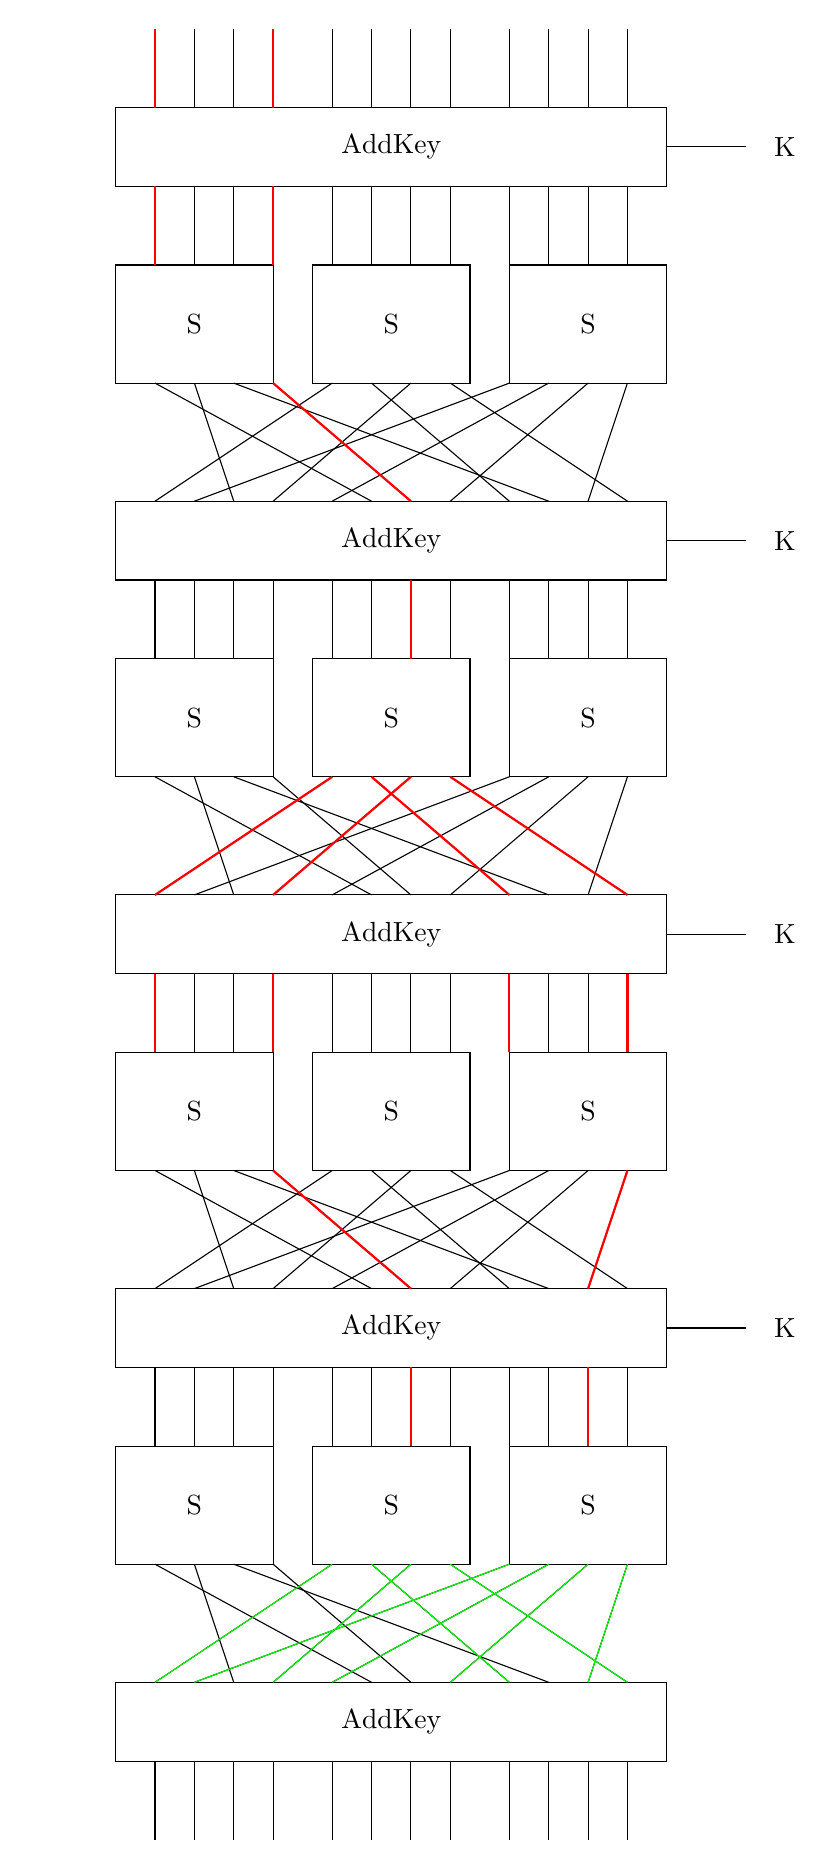
\begin{tikzpicture}[scale=0.50]
            \foreach \x in {1, 2, 3, 4, 5.5, 6.5, 7.5, 8.5, 10, 11, 12, 13}
                \draw[-] (\x, 33) -- (\x, 31);
            \foreach \y in {31, 21, 11, 1}{
                \node at (-2, \y-1) {};
                \draw (0, \y) rectangle (14, \y-2);
                \node at (7, \y-1) {AddKey};
                \draw[-] (14, \y-1) -- (16, \y-1);
                \node at (17, \y-1) {K};
                \foreach \x in {0, 5, 10}{
                    \draw (\x, \y-4) rectangle (\x + 4, \y-7);
                    \node at (\x + 2, \y-5.5) {S};
                }
                \foreach \x in {1, 2, 3, 4, 5.5, 6.5, 7.5, 8.5, 10, 11, 12, 13}
                    \draw[-] (\x, \y-2) -- (\x, \y-4);
                \draw[-] (1, \y-7) -- (6.5, \y-10);
                \draw[-] (2, \y-7) -- (3, \y-10);
                \draw[-] (3, \y-7) -- (11, \y-10);
                \draw[-] (4, \y-7) -- (7.5, \y-10);
                \draw[-] (5.5, \y-7) -- (1, \y-10);
                \draw[-] (6.5, \y-7) -- (10, \y-10);
                \draw[-] (7.5, \y-7) -- (4, \y-10);
                \draw[-] (8.5, \y-7) -- (13, \y-10);
                \draw[-] (10, \y-7) -- (2, \y-10);
                \draw[-] (11, \y-7) -- (5.5, \y-10);
                \draw[-] (12, \y-7) -- (8.5, \y-10);
                \draw[-] (13, \y-7) -- (12, \y-10);
            }
            \draw (0, -9) rectangle (14, -11);
            \node at (7, -10) {AddKey};
            \foreach \x in {1, 2, 3, 4, 5.5, 6.5, 7.5, 8.5, 10, 11, 12, 13}
                \draw[-] (\x, -11) -- (\x, -13);
            
            \draw[-, red, thick] (1, 33) -- (1, 31);
            \draw[-, red, thick] (4, 33) -- (4, 31);
            \draw[-, red, thick] (1, 29) -- (1, 27);
            \draw[-, red, thick] (4, 29) -- (4, 27);

            \draw[-, red, thick] (4, 24) -- (7.5, 21);
            \draw[-, red, thick] (7.5, 19) -- (7.5, 17);

            \draw[-, red, thick] (5.5, 14) -- (1, 11);
            \draw[-, red, thick] (6.5, 14) -- (10, 11);
            \draw[-, red, thick] (7.5, 14) -- (4, 11);
            \draw[-, red, thick] (8.5, 14) -- (13, 11);

            \draw[-, red, thick] (1, 9) -- (1, 7);
            \draw[-, red, thick] (4, 9) -- (4, 7);
            \draw[-, red, thick] (10, 9) -- (10, 7);
            \draw[-, red, thick] (13, 9) -- (13, 7);

            \draw[-, red, thick] (4, 4) -- (7.5, 1);
            \draw[-, red, thick] (13, 4) -- (12, 1);

            \draw[-, red, thick] (7.5, -1) -- (7.5, -3);
            \draw[-, red, thick] (12, -1) -- (12, -3);

            \draw[-, green] (5.5, 1-7) -- (1, 1-10);
            \draw[-, green] (6.5, 1-7) -- (10, 1-10);
            \draw[-, green] (7.5, 1-7) -- (4, 1-10);
            \draw[-, green] (8.5, 1-7) -- (13, 1-10);
            \draw[-, green] (10, 1-7) -- (2, 1-10);
            \draw[-, green] (11, 1-7) -- (5.5, 1-10);
            \draw[-, green] (12, 1-7) -- (8.5, 1-10);
            \draw[-, green] (13, 1-7) -- (12, 1-10);
        \end{tikzpicture}
    \end{center}
    \caption{Propagation de différence dans le SPN}
    \label{chemin}
\end{figure}

\section*{Attaque par saturation sur l'AES}

\begin{lemma*}
    Soit $l$ un entier tel que $l \geq 2$, alors :
    \begin{displaymath}
        \bigoplus_{u \in \{0,1\}^l} u = 0
    \end{displaymath}
\end{lemma*}

\begin{proof}
    Nous démontrerons le lemme précédent par récurrence. Considérons le cas où $l = 2$, l'ensemble
    des mots $u \in \{0,1\}^2$ est le suivant :
    \begin{displaymath}
        \begin{array}{c|cc}
            & 0 & 1 \\ \hline
            0 & 00 & 01 \\ 
            1 & 10 & 11 \\
        \end{array}
    \end{displaymath}
    Si l'on réalise un Xor sur l'ensemble de ce mots on a ce qui suit :
    \begin{displaymath}
        00 \oplus 01 \oplus 11 \oplus 10 = 10 \oplus 10 = 00
    \end{displaymath}

    Considérons à présent que $\bigoplus_{u \in \{0,1\}^n} u = 0$ et intéressons nous au résultat de
    $\bigoplus_{u \in \{0,1\}^{n+1}} u$. Pour ce faire, remarquons tout d'abord que : 
    \begin{displaymath}
        \bigoplus_{u \in \{0,1\}^l} = \concat_{j = 1}^{l} \bigoplus_{u \in \{0,1\}^l} u_j
    \end{displaymath}
    avec $u_i$ le $i^e$ bit du mot $u$ et $\concat$ l'opération de concaténation. Remarquons ensuite
    que \begin{displaymath}
        U_{n+1} = \{0 \concat U_n, 1 \concat U_n\}
    \end{displaymath}
    autrement dit, l'ensemble des mots binaires de taille $n+1$ est égale à l'ensemble des mots
    binaires de taille $n$ préfixé de $0$ et de $1$. On peut alors écrire ce qui suit :
    \begin{displaymath}
        \begin{array}{rcll}
            \bigoplus_{u \in \{0,1\}^{n+1}} & = & \bigoplus_{u \in \{O,1\}^n} 1 \concat u \oplus \bigoplus_{u \in \{0,1\}^n} 0 \concat u & \\
                                            & = & \bigoplus_{j = 1}^{2^n} 10^n + \bigoplus_{j=1}^{2^n} 0^{n+1} & \\
                                            & = & \bigoplus_{j = 1}^{2^n} 10^n & \\
                                            & = & 0 & \quad \mbox{ car }2^n\mbox{ est pair }\\
        \end{array}
    \end{displaymath}
    CQFD
\end{proof}

Le cas particulier où $l=8$ est donc vrai lui aussi.

\subsection*{Forme des messages au fur et à mesure des rondes}

Le principe de l'attaque par saturation est de sélectionner un octet du message $M$ en entrée et de
lui faire prendre toutes les valeurs possibles, les 15 autres octets prenant toujours la même
valeur. On obtient alors un jeu de 256 messages que nous appellerons $N$. On regarde alors comment
évoluent les messages considérés lors de leur passage dans l'algorithme.

Quelques conventions : \begin{itemize}
    \item $a$ : un octet noté $a$ prend les 256 valeurs possibles, donc pour chaque message $M_i$ de
        $N$, la valeur de l'octet noté $a$ est différente
    \item $c$ : un octet noté $c$ est un octet dont la valeur est identique pour tous les messages
        $M_i$ de $N$. Il est important de noter que deux octets notés $c$ n'ont pas forcément même
        valeur.
    \item $s$ : un octet noté $s$ est un octet pour lequel nous connaissons la valeur du Xor : si
        l'on effectue un Xor sur les 256 messages de $N$, on connaît le résultat pour cet octet.
\end{itemize}

L'ensemble des messages est alors représentable par un seul en entrée de la première ronde :
\begin{displaymath}
    \begin{array}{|c|c|c|c|} \hline
        a & c & c & c \\ \hline
        c & c & c & c \\ \hline
        c & c & c & c \\ \hline
        c & c & c & c \\ \hline
    \end{array}
\end{displaymath}

\subsubsection*{Après la première ronde}

Au cours la première ronde d'AES, 5 opérations sont effectuées : 
\begin{enumerate}
    \item AddRoundKey
    \item SubByte
    \item ShiftRows
    \item MixColumns
    \item AddRoundKey
\end{enumerate}

Les opérations AddRoundKey et SubByte ne modifie pas la structure des messages :
\begin{itemize}
    \item Un octet prenant toutes les valeurs en entrée prendra toutes les valeurs en sortie du fait
        de la bijectivité de ces fonctions
    \item Un octet ayant toujours la même valeur sur $N$ aura une valeur différente de la valeur
        initiale, mais aura une valeur finale identique sur tous les messages de $N$
\end{itemize}
L'opération ShiftRows ne modifiera pas non plus la structure des messages puisque la première ligne
ne subissant aucune rotation, l'octet saturé ne changera pas de place. L'opération MixColumns, quant
à elle, va propager la saturation de l'octet saturé à la colonne à laquelle il appartient. Ceci est
dû au produit matriciel de chacun des messages par la matrice $G$ suivante : \begin{displaymath}
    \left [ 
        \begin{array}{cccc}
            2 & 3 & 1 & 1 \\
            1 & 2 & 3 & 1 \\
            1 & 1 & 2 & 3 \\
            3 & 1 & 1 & 2 \\
        \end{array}
    \right ]
\end{displaymath}
Tous les octets de la première colonne prennent donc la valeur : $ 2a + 3c + c + c mod (x^4 + 1)$,
$c$ représentant un octet constant et $a$ un octet saturé, les octets de la première colonne
devienne donc tous saturés.
Enfin comme précédemment, AddRoundKey ne modifie pas la structure des blocs de message et donc les
messages en sortie sont de la forme :
\begin{displaymath}
    \begin{array}{|c|c|c|c|} \hline
        a & c & c & c \\ \hline
        a & c & c & c \\ \hline
        a & c & c & c \\ \hline
        a & c & c & c \\ \hline
    \end{array}
\end{displaymath}

\begin{lemma*}
    Si l'on appelle $C^{(1)}$ l'ensemble des chiffrés de $N$ après la première ronde, et donc
    $C_i^{(1)}$ le chiffré de $M_i$ après la première ronde, alors :
    \begin{displaymath}
        \bigoplus_{i=0}^{255}C_i^{(1)} = 0
    \end{displaymath}
\end{lemma*}

\begin{proof}
    La preuve est presque évidente et donc très rapide. D'après le lemme précédent,
    $\bigoplus_{i=0}^{255} a = 0$ puisque $a$ est un octet saturé et donc $a = \{0,1\}^8$.
    De plus $\bigoplus_{i=0}^{255} c = \bigoplus_{j=0}^{127} \bigoplus_{i=0}^1 c =
    \bigoplus_{j=0}^{127} 0 = 0$.

    On a alors :
    \begin{displaymath}
        \begin{array}{rcl}
            \bigoplus_{i=0}^{255} C_i^{(1)} & = & \bigoplus_{i=0}^{255} a \concat_{j=1}^{15} \bigoplus_{i=0}^{255} c\\
                                            & = & 0 \concat_{j=1}^{15} 0 \\
                                            & = & 0 \\
        \end{array}
    \end{displaymath}
    CQFD.
\end{proof}

\subsubsection*{Après la seconde ronde}

La seconde ronde est identique à la première si l'on supprime la première opération AddRoundKey. De
la même manière que précédemment, SubByte ne modifie pas la structure des messages.
Cette fois ci, l'opération ShiftRows va entraîner un déplacement de certains octets actifs de la
manière suivante :
\begin{displaymath}
    \begin{array}{|c|c|c|c|} \hline
        a & c & c & c \\ \hline
        c & c & c & a \\ \hline
        c & c & a & c \\ \hline
        c & a & c & c \\ \hline
    \end{array}
\end{displaymath}
Et de la même manière que précédemment, l'opération MixColumns va propager la saturation des octets
saturés aux colonnes les contenant, donc aux quatre colonnes des messages. L'opération AddRoundKey
n'ayant aucune incidence sur la structure, on obtient alors :
\begin{displaymath}
    \begin{array}{|c|c|c|c|} \hline
        a & a & a & a \\ \hline
        a & a & a & a \\ \hline
        a & a & a & a \\ \hline
        a & a & a & a \\ \hline
    \end{array}
\end{displaymath}

\begin{lemma*}
    \begin{displaymath}
        \bigoplus_{i=0}^{255} C_i^{(2)} = 0
    \end{displaymath}
\end{lemma*}

\begin{proof}
    Tous les octets sont saturés donc leur somme\footnote{Par abus de langage, et par facilité,
        voire fainéantise de l'auteur, la somme d'octet correspond à un ou exclusif des octets
    considérés.} est nulle d'après le pénultième lemme. La concaténation de la somme des octets
    a, elle aussi, pour résultat $0$.
\end{proof}

\subsubsection*{Après la troisième ronde}

L'opération importante de la troisième ronde est le MixColumns, puisque c'est elle qui va "faire en
sorte" que les octets ne soient plus forcément saturés. Avant cette opération, la somme des messages
est nulle puisque tous les octets sont saturés puisque SubByte ne modifie pas la structure des
messages et ShiftRows ne fait qu'appliquer une rotation sur les rangées de la colonne.

\begin{thrm*}
    Après l'opération de MixColumns la somme des messages est toujours nulle.
\end{thrm*}

\begin{proof}
    Prenons la formulation mathématiques du MixColumns, appelons $v_{ij}$ l'octet se trouvant à
    l'intersection de la rangée $i$ et de la colonne $j$ après l'opération MixColumns, et appelons
    $u_{ij}$ l'octet à la même position avant l'opération MixColumns. On peut alors écrire :
    \begin{displaymath}
        \begin{array}{rrcl}
            & b_{ij} & = & 2 a_{ij} + 3 a_{i+1 j} + a _{i+2 j} + a_{i+2 j} \\
            \Rightarrow & \bigoplus_{k=0}^{255} b_{ij} & = & \bigoplus_{k=0}^{255} ( 2 a_{ij} + 3 a_{i+1 j} + a _{i+2 j} + a_{i+2 j} )\\
                        & & = & 2 \bigoplus_{k=0}^{255} a_{ij} \oplus 3 \bigoplus_{k=0}^{255} a_{i+1j} \oplus \bigoplus_{k=0}^{255} a_{i+2j} \oplus \bigoplus_{k=0}^{255} a_{i+2j} \\
                        & & = & 0 \oplus 0 \oplus 0 \oplus 0 \\
                        & & = & 0 \\
        \end{array}
    \end{displaymath}
    La somme de chaque octet est nulle, donc la somme des messages est nulle.
    CQFD
\end{proof}

\subsection*{L'attaque}

\subsubsection*{AES à quatre tours}

A la fin de la troisième ronde, la somme des messages est nulle. La dernière ronde ne comportant pas
de MixColumns, il est alors possible d'attaquer tous les octets de la clé un par un. En effet,
pour chaque message chiffré, il suffit d'inverser la dernière ronde et de vérifier que la somme des
octets des messages obtenus est nulle. Si tel est le cas, alors il y a de (très) grandes chances que
l'octet trouvé soit le bon. Dans l'éventualité ou plusieurs octets différents permettraient de
vérifier cette propriété, il suffit alors de refaire la même manipulation en saturant un octet
différent de celui qui a été choisi précédemment.

\subsubsection*{AES à 5 tours}

Je pourrais recracher ce que j'ai lu à ce sujet, comme quoi il suffit de deviner 4 bits de la clé et
procéder à une attaque de la même manière que précédemment, mais je n'ai pas bien compris en quoi
cela fonctionne et comment cela fonctionne. Si vous avez un ou plusieurs documents pouvant me
permettre de comprendre, je suis preneur.

\subsubsection*{Le code}

L'attaque sur AES à 4 tours ne fonctionne pas. Il y a plusieurs possibilités à ceci :
\begin{itemize}
    \item une erreur d'implémentation complètement stupide qui m'empêche d'arriver au résultat
        attendu
    \item une mauvaise compréhension du code fourni et donc une mauvaise implémentation de l'attaque
    \item dans l'éventualité ou dernière clé de ronde trouvée soit le bonne, il peut y avoir une
        erreur dans l'implémentation de la fonction chargée de retrouver la clé initiale à partir de
        la clé de ronde
    \item ou peut être tout simplement, une mauvaise compréhension de l'attaque
\end{itemize}


\end{document}

